\documentclass{beamer}
%\usefonttheme{serif}
\usepackage{listings}

\setbeamertemplate{bibliography item}{}

%\setbeamerfont{title}{family=\rm\addfontfeatures{Scale=1.18, Numbers={Lining, Proportional}}}

\title[acoustics] % (optional, only for long titles)
{Three Dimensional Room Acoustics Models}
\subtitle{and Optimising for Performance on the GPU}
\author[Author] % (optional, for multiple authors)
{Jacob Josiah Webber}
\date[4 April 2017] % (optional)
{Project Preparation Presentation}
\subject{HPC}


\begin{document}
\frame{\titlepage}

  \begin{frame}
     \frametitle{Introduction}
     This talk aims to answer the following questions:
     \begin{itemize}
     \item What is sound?
     \item How do the spaces we hear them in affect this sound?
     \item What methods currently exist to simulate this?
     \item Why would we want to simulate this?
     \item How will I try to improve these?
     \end{itemize}
  \end{frame}



  \begin{frame}
    \frametitle{Sound}
    \framesubtitle{What is it?}
    \begin{block}{From Wikipedia}
    ``In physics, sound is a vibration that propagates as a typically audible mechanical wave of pressure and displacement, through a transmission medium such as air or water.''
    \end{block}
    \nocite{feynman}
    \begin{block}{From my undergraduate degree}
    \begin{equation}
    \nabla^{2} \textbf{p} - \frac{1}{{c^2 }}\frac{{\partial ^2 \textbf{p}}}{{\partial t^2 }} = 0
    \end{equation}
    \end{block}
  \end{frame}
  
  
  \begin{frame}
  \frametitle{Room acoustics}
  \begin{itemize}
  \item The physical properties of rooms affects how we hear sound.
  \item Sound reverberates off walls/objects.
  \item Some rooms echo, some sound dry.
  \item Backwards: If we know physical properties can we derive the sound?
  \end{itemize}
  \end{frame}
  
  
\begin{frame}
\frametitle{The wave equation}
$$\frac{\partial ^2 \textbf{p}}{\partial x^2 } - \frac{1}{{c^2 }}\frac{{\partial ^2 \textbf{p}}}{{\partial t^2 }} = 0$$
where $\textbf{p}$ is pressure deviation and $c$ is speed of sound in medium.
\linebreak
\begin{itemize}
\item Very familiar to those who have studied physics
\item It, and its application to acoustics, are derivable from first principles.
\item Solving for $\textbf{p}$ gives us acoustic properties of a system.
\item Solving this analytically for complex systems is not possible.
\end{itemize}    
\end{frame}

\begin{frame}
\frametitle{FTDT}
\framesubtitle{Finite-difference time-domain method}
Finite difference methods are a way of approximating and discretising differential equations so that they can be solved numerically.
\linebreak

Effectively turns solving differential equation into a large stencilling operation.
\linebreak

Simple 1 dimensional example:
$$ \frac{df(x)}{dx} \approx \frac{f(x+h) - f(x-h)}{2h} $$
\end{frame}


\begin{frame}
\frametitle{Memory considerations}
For stencilling operations, memory access is the bottleneck.
\begin{itemize}
\item Accurate models need a lot of points to model a room.
\item High memory bandwidth means GPUs are used - limited memory.
\item Standard 3d arrays are cuboid.
\item Due to memory layout, neighbouring points in space will always be far apart in memory.
\end{itemize}
\end{frame}
 
\begin{frame}
\begin{figure}
\centering
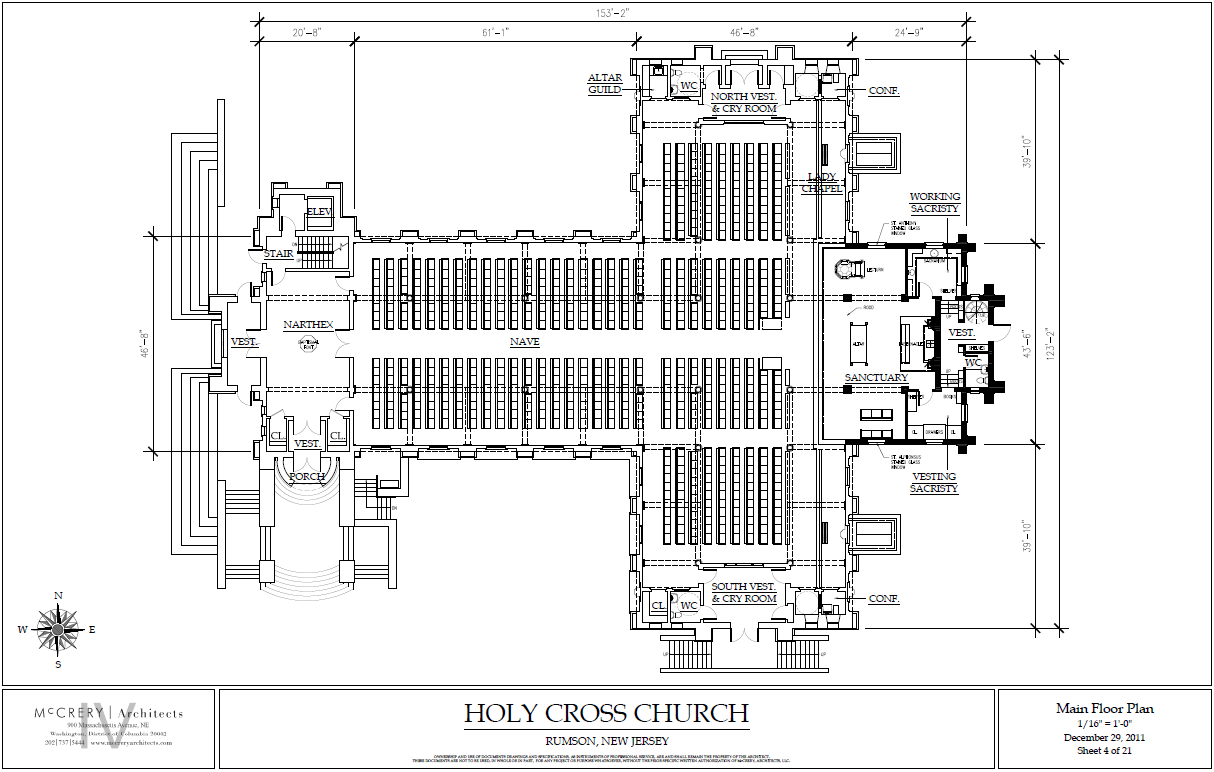
\includegraphics[width=\textwidth]{../diagrams/church}
\label{church}
\end{figure}
\end{frame}


\begin{frame}
\frametitle{The Proposal}
Use an array of structs instead!
\begin{itemize}
\item Store enough points for CUDA kernel to operate on.
\item Only store structs with at least one point inside the room.
\item Experiment with different sized arrays within the struct to see if caching benefits can be yielded.
\end{itemize}
\end{frame}  
  
\begin{frame}[fragile]
\frametitle{The Struct}

\begin{lstlisting}[caption=First 2d example]

struct linked_struct {
    int up;
    int down;
    int left;
    int right;
    float value[X][Y];
    float old_value[X][Y];
    char inside[X][Y];
};
\end{lstlisting}
\end{frame}

\begin{frame}
\begin{figure}
\centering

\includegraphics[height=0.75\textheight]{../diagrams/diagram}
\caption{Diagram showing unit square rotated by $\theta$ within bounding square, where $x$ is the side of the bounding square.}
\label{spr}
\end{figure}
\end{frame}


  \begin{frame}
     \frametitle{The End}
     This talk aimed to answer the following questions:
     \begin{itemize}
     \item What is sound?
     \item How do the spaces we hear them in affect this sound?
     \item What methods currently exist to simulate this?
     \item Why would we want to simulate this?
     \item How will I try to improve these?
     \end{itemize}
  \end{frame}



\begin{frame}
\frametitle{References}
\bibliographystyle{plain}
\begin{thebibliography}{}

\bibitem{feynman}
Richard Feynman,  1969, 
\textit{Lectures in Physics, Volume 1,}
Addison Publishing Company, Addison



\end{thebibliography}
\end{frame}

% etc
\end{document}